\documentclass{article}

% if you need to pass options to natbib, use, e.g.:
%     \PassOptionsToPackage{numbers, compress}{natbib}
% before loading neurips_2019

% ready for submission
% \usepackage{neurips_2019}

% to compile a preprint version, e.g., for submission to arXiv, add add the
% [preprint] option:
%     \usepackage[preprint]{neurips_2019}

% to compile a camera-ready version, add the [final] option, e.g.:
     \usepackage[final]{neurips_2019}

\usepackage{amsmath}
\usepackage{algorithm}
\usepackage[noend]{algpseudocode}

\usepackage[pdftex]{graphicx}
% to avoid loading the natbib package, add option nonatbib:
%     \usepackage[nonatbib]{neurips_2019}

\usepackage[utf8]{inputenc} % allow utf-8 input
\usepackage[T1]{fontenc}    % use 8-bit T1 fonts
\usepackage{hyperref}       % hyperlinks
\usepackage{url}            % simple URL typesetting
\usepackage{booktabs}       % professional-quality tables
\usepackage{amsfonts}       % blackboard math symbols
\usepackage{nicefrac}       % compact symbols for 1/2, etc.
\usepackage{microtype}      % microtypography

\title{A crossover code for high-dimensional composition}

% The \author macro works with any number of authors. There are two commands
% used to separate the names and addresses of multiple authors: \And and \AND.
%
% Using \And between authors leaves it to LaTeX to determine where to break the
% lines. Using \AND forces a line break at that point. So, if LaTeX puts 3 of 4
% authors names on the first line, and the last on the second line, try using
% \AND instead of \And before the third author name.

\author{%
  Rich Pang\\
  Computational Neuroscience Center\\
  University of Washington\\
  Seattle, WA 98195\\
  \texttt{rpang at uw dot edu} \\
  % examples of more authors
  % \And
  % Coauthor \\
  % Affiliation \\
  % Address \\
  % \texttt{email} \\
  % \AND
  % Coauthor \\
  % Affiliation \\
  % Address \\
  % \texttt{email} \\
  % \And
  % Coauthor \\
  % Affiliation \\
  % Address \\
  % \texttt{email} \\
  % \And
  % Coauthor \\
  % Affiliation \\
  % Address \\
  % \texttt{email} \\
}

\begin{document}

\maketitle

\begin{abstract}
We present a novel method for encoding compositional information by recursively interweaving high-dimensional (HD) random vectors. Inspired by chromosomal crossover, a fraction of one vector's components are masked out and replaced by those from another, via a context-dependent mask. Unlike most HD computing schemes, "crossover" codes highly overlap their base elements' and sub-structures' codes yet without sacrificing relational information, allowing direct element recovery and decoding by greedy reconstruction. Crossover is mathematically tractable and has several properties desirable for robust, flexible representation.
\end{abstract}

\section{Introduction}

A common problem faced by intelligent systems is how to encode objects of variable complexity in fixed dimensions. Ideally, similar objects should have similar codes, new object codes should not degrade existing ones, and there should be no hard object complexity limit. Distributing codes across high-dimensional (HD) vectors yields robustness and potential flexibility and generalization \cite{Hinton:1984, Mikolov:2013}, but how does one encode order or binding relations (key to composition) in such a code, e.g. to distinguish AB vs BA or (AB, CD) vs (AC, CB), respectively? While trained networks have some implicit capacity for this \cite{language network}, it is unclear (1) how such networks might encode complexity beyond that in their training data, and (2) how to quantify internal network representations. An alternative approach, known as HD computing (HDC), is to assign \textit{random} vector codes to a set "base" elements of the data (e.g. symbols), and rules for composing these into richer data structures (e.g. words) \cite{Plate, Kanerva, Gayler}. HDC's advantages are (1) random HD vectors are nearly orthogonal with high probability, enabling a large element codebook, (2) there is no hard limit on data complexity, and (3) encoding is often mathematically tractable. Thus, while a useful system would of course require some training on environment statistics, HDC provides a compelling blueprint for representational flexibility.

Most HDC schemes are based on relational codes that little overlap their element codes (e.g. $AB$'s code is distinct from $A$'s and $B$'s), yet from which the relations can be readily recovered. Examples of typical relation-encoding operations include circular convolution \cite{Plate}, permutation \cite{Sahlgren, Gayler}, or matrix multiplication \cite{Gosmann}. Because of this non-overlap, elements cannot be directly recovered from the relation code (although see \cite{Rachkovskij:2001}), and such a scheme conflicts with our desire that $AB$ should resemble $A$ more than $C$. Here, we present a new way (to our knowledge) to encode relations (and arbitrary compositions), where two vectors $X^A$ and $X^B$ are ordered or bound by masking out a fraction of $X^A$'s components and replacing them with those from $X^B$, analogous to chromosomal crossover, with relational information encoded in a context-dependent mask $\mu(X^A, X^B)$. "Crossover" composition codes highly overlap with the substructures and base elements used to build them, allowing direct recovery of elements and decoding by greedy reconstruction. Further, they distribute information evenly across components and have statistics invariant to object complexity, suggesting utility for robust intelligent systems. We focus on sequences first, then generalize to binding and trees.

\section{Sequence encoding}

Let $X$ be a vector of $N$ components, each of which can take any of $Z$ states, $x_j \in G \equiv \{1,...,Z\}$, and let $d(X^A, X^B)$ be the Hamming distance from $X^A$ to $X^B$. For a symbol sequence $Y = (y_1, ..., y_L)$, where $y_t \in D \equiv \{1, ..., M\}$, we establish a mapping from $Y$ to $X^Y$ as follows:

First sample a codebook $C \equiv \{X^1, ..., X^M, X^*\}$, where $X^*$ is a "start code", and $x^j$ are i.i.d. across all components and codes and sampled uniformly from $G$. Next sample a mask function $\mu$, an $N \times M^{2N}$ matrix with i.i.d. real-valued elements from $\textrm{Uniform}(0, 1)$, which we reference as $\mu_j(X^A, X^B)$. In practice, columns of $\mu$ can be sampled "as needed" with a hash function.

Using $C$ and $\mu$ we construct sequence codes as described in Algorithm 1 and Figure 1:, symbol codes are recursively woven into the constructed code by replacing a fraction of the current code's components with those from the symbol code; which specific components are replaced depends on the current and symbol codes (the context). We decrease the fraction as $1/(t+1)^\gamma$, for $\gamma \geq 1$ to prevent exponential decay of the first symbol's similarity to the final code.

\begin{algorithm}
\caption{Sequence Encoding}

\begin{algorithmic}[0]
\Function{CrossoverSeq}{$X^A, X^B; t$}

\State $mask \gets (\mu(X^A, X^B) < 1/(t+1)^\gamma) \quad$  \# context-dependent mask w/ about $1/(t+1)^\gamma$ 1's
\State $X^{AB} \gets X^A$
\State $X^{AB}[mask] \gets X^B[mask] \quad$  \# replace $X^A$'s masked components $X^B$'s

\State \textbf{return} $X^{AB}$
\EndFunction

\Function{EncodeSequence}{$Y$}
\State $X^Y \gets X^*$
\For{$t \in 1, ..., |Y|$}

\State $X^Y \gets CrossoverSeq(X^Y, X^{y_t}, t)$

\EndFor

\State \textbf{return} $X^Y$
\EndFunction

\end{algorithmic}
\end{algorithm}

\begin{figure}
  \centering
  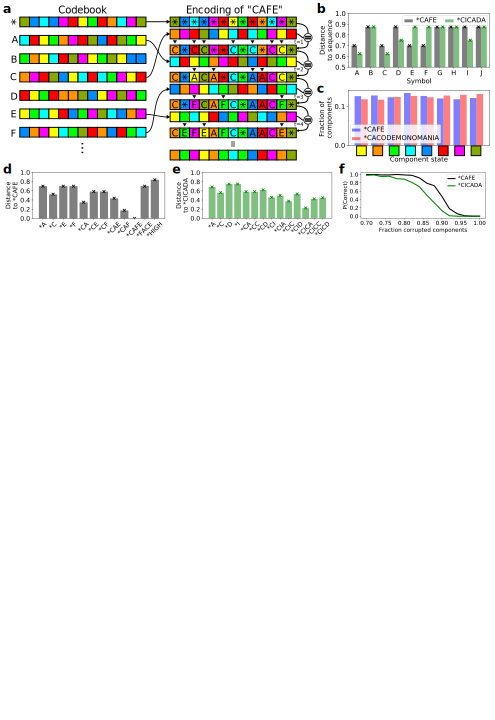
\includegraphics{1_sequences.pdf}
  \caption{Sequence encoding via crossover ($N=1024, Z=8, M=26, \gamma=1$). (a) Example encoding of CAFE; colors are states, inscribed symbols are visual aids, not used by the algorithm. (b) Sequence-symbol code distances. (c) State distributions for a short and long sequence. (d, e) Distances of CAFE's and CICADA's code to other sequence codes. (f) Decoding vs code corruption.}
\end{figure}

\begin{figure}
  \centering
  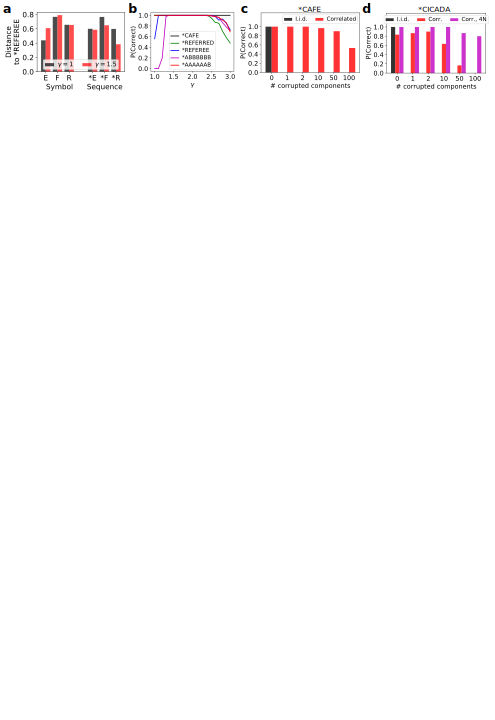
\includegraphics{2_gamma.pdf}
  \caption{Crossover modifications. (a) Distance of *REFEREE to symbols/sequences for two $\gamma$. (b) Decoding vs. $\gamma$ for several sequences. (c) Decoding of *CAFE vs corrupted encoding for i.i.d. and correlated $\mu$. (d) Decoding of *CICADA for i.i.d., correlated $\mu$, and correlated $\mu$ with increased $N$.}
\end{figure}

\begin{figure}
  \centering
  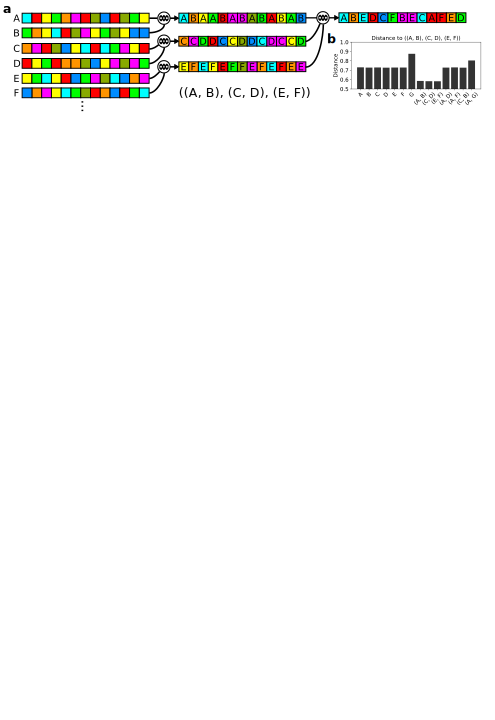
\includegraphics{3_trees.pdf}
  \caption{Tree encoding via crossover ($N=1024, Z=8, M=26$). (a) Example encoding of (AB, CD, EF). (b) Similarity between final code and element and sub-tree codes.}
\end{figure}

\section{Discussion}

While an intelligent agent must learn environmental statistics to some extent, it can be desirable to certain computations built-in instead of learned from scratch \cite{Zador:2019}. Flexible composition is particularly useful, since lets an agent compute with novel objects/events if they are composed of familiar elements \cite{Jackendoff, Gayler}: it would benefit an autonomous vehicle to be able to automatically generate and manipulate a representation of "child on scooter behind car in front of bus", even if previously it had only worked with any of the constituent elements in isolation. Computationally, basing neural network training protocols on built-in HDC codes for composition \cite{Plate} to learn knowledge graphs yielded more efficient computation, easy training, and high scalability \cite{Nickel:2015}. It stands to reason that improving HDC codes may improve network training further still.

As it was discovered early that sums of HD random vectors could encode \textit{sets}, due to high similarity to their components \cite{Bloom:1970, Anderson:1973, Plate:1994}, most HDC work has focused on relations, like sequences or bindings. Perhaps best known are holographic representations \cite{Plate:1995}, where element vectors are bound by circular convolution. Additional proposed binding operations are base on XOR (for binary vectors) \cite{Kanerva:1996}, permutation \cite{Gayler:1998}, or matrix multiplication \cite{Gosmann:2019}. To encode order, convolution can be slightly modified \cite{Murdock:1983, Plate:1995} or prior to summing each element can first be tagged via permutation \cite{Sahlgren:2008} or binding to location tokens \cite{Kanerva:1996}. While such schemes preserve recoverable relational information, the composite vectors are dissimilar to their elements, preventing recovery of the elements from their similarity to the composite vector. An exception is "context-dependent thinning" (CDT), where elements are bound by summing them, then "stamping" them with a set of zeros dependent on the sum \cite{Rachkovskij:2001}; while the stamp shape retains binding information, however, information beneath its imprint is discarded, partially degrading the desired similarities; and it is not clear how CDT could be used to construct recursive sequence codes without early elements' similarities decaying exponentially. The scheme presented in this paper, termed "crossover", overcomes these limitations, preserving similarity to element and sub-structure codes without sacrificing relational information; further, the sequence code automatically prevents early element similarities from being lost, improving decodability. Beyond this, crossover codes have i.i.d. information across the vector components, and code statistics are invariant to object complexity. Crossover might thus be a useful blueprint for a robust cognitive system capable of working with arbitrary objects.

We close by discussing HDC's potential implementation in biological neural networks. Of key interest is the working memory (WM) system, which must generate and maintain representations of novel objects (e.g. a never-before-heard question) on the fly. It has been hypothesized that information persists in WM through persistent patterns of neural activity \cite{Chaudhuri Nat Neuro}. While certain networks can support the combinatorial persistent patterns required for composition \cite{papers from CSHL application}, how they might carry meaning is little understood. HDC suggests an answer: by decomposing such patterns into independent components and assigning these to the components of an HDC vector, one could map the space of HDC representations to plausible neural activity, so that the latter inherited HDC's representational flexibility. This could provide a robust, expressive reservoir of neural representations that could be manipulated by recurrent computations.

\subsubsection*{Acknowledgments}

Use unnumbered third level headings for the acknowledgments. All acknowledgments
go at the end of the paper. Do not include acknowledgments in the anonymized
submission, only in the final paper.

\section*{References}

References follow the acknowledgments. Use unnumbered first-level heading for
the references. Any choice of citation style is acceptable as long as you are
consistent. It is permissible to reduce the font size to \verb+small+ (9 point)
when listing the references. {\bf Remember that you can use more than eight
  pages as long as the additional pages contain \emph{only} cited references.}
\medskip

\small

[1] Alexander, J.A.\ \& Mozer, M.C.\ (1995) Template-based algorithms for
connectionist rule extraction. In G.\ Tesauro, D.S.\ Touretzky and T.K.\ Leen
(eds.), {\it Advances in Neural Information Processing Systems 7},
pp.\ 609--616. Cambridge, MA: MIT Press.

[2] Bower, J.M.\ \& Beeman, D.\ (1995) {\it The Book of GENESIS: Exploring
  Realistic Neural Models with the GEneral NEural SImulation System.}  New York:
TELOS/Springer--Verlag.

[3] Hasselmo, M.E., Schnell, E.\ \& Barkai, E.\ (1995) Dynamics of learning and
recall at excitatory recurrent synapses and cholinergic modulation in rat
hippocampal region CA3. {\it Journal of Neuroscience} {\bf 15}(7):5249-5262.

\end{document}
